
% 和文概要
\begin{abstract}
実世界と情報世界を接続し,大学の研究室内での情報共有を便利にするシステムを作成した.本システムには3つの機能がある.1つ目の機能は,物体を識別する機能である.研究室内では各人が共有物を使って工作や勉強を行っている.また,私物を持ち込む場合もある.しかしそれらの物品は小型な場合が多く,RFIDやバーコードなどのタグを付けると実際の作業の邪魔になってしまう.そこで本研究では,重さを用いて物体を認識するしくみを作成した.2つ目の機能は,物に対してweb上から複数人で情報を付与する機能である.研究室内にある機材には付箋や書き込み以上の注釈を書きたい場合もあるし,写真や映像で使い方を説明したい事もある.3つ目の機能は,web上での情報更新を実世界に通知する機能である.私たちは常にラップトップコンピュータを開いているわけではなく,移動したり,他の作業をしていたりする.一般的に研究室の全員に情報を共有する方法としてメーリングリストを使う事が多いと思うが,そうではなくweb上の情報を主として,その更新通知のみを行うもっと軽い方法が必要だと考えた.
\end{abstract}

% 英文概要
\begin{eabstract}
english english english
\end{eabstract}

\maketitle

% 本文はここから始まる
\section{はじめに}\label{sec:Introduction}
実世界と情報世界を接続する時に,主に3つの問題がある.物とweb上の知識のリンク方法と,web上でいかに知識を共同編集し,その変化をユーザーに通知するかという事である.本論文で説明するシステムは,大学の研究室という環境において工具や道具などの物体からweb上の知識へと簡単にリンクさせる事ができ,またweb上での知識の共同編集し,知識の編集過程を研究室のメンバーに通知する事ができる.

大学の研究室にある特殊な工具についての情報をweb上の情報とリンクさせる際に,まずユーザにとって物の正確な名前がわからないので検索できない事が問題になる.その問題を解決する方法として,
(ここに関連研究.バーコードの例,RFIDの例,画像検索の例,お茶大のWISS)
本研究では,物の持つ物理的な特徴である重さを用いて,物体を認識する事にした.重さを使う事には以下の2つの利点がある.1つ目は,使いやすい事である.バーコードの様に正しい向きでスキャンする必要が無く,ただ量りに乗せるだけで良く,また画像検索と異なり正しい向きで認識させる必要もない.2つ目は,物体が最初から持っている物理的特徴を利用するので,物にタグを貼り付ける必要が無い事である.

web上での知識の共同編集方法の代表的な物としてはwikiが挙げられる.MediaWiki\cite{mediawiki}等の多くのwikiには更新通知機能があるが,その通知方法はメールで定期的にまとめて通知されるものだ.しかし,研究室のメンバーはそれぞれがパソコンに向かっていたり,移動していたり,電子工作をしていたりする.つまり既存のwikiとその更新通知システムは,多様な状態を持つユーザに対してリアルタイムな更新通知ができない.本研究では,webサービスとして実装されたアウトラインエディタと,様々なメディアに適切なフォーマットで更新通知するシステムによりこの問題を解決した.


\section{システムの概要}
本システムには,1.重さにより物体を認識する機能,2.物についてweb上で文書を共同編集する機能,3.web上の文書の更新をユーザに適切に通知する機能 がある.ここでは,実装したシステムの使い方について説明する.

ユーザは身の回りの工具や道具をはかりに乗せる.(図:\ref{fig:sensor})はかりは重さを計測し,物体と重さのデータベースを検索する.該当する重さが存在すれば,はかりが接続されたコンピュータにウェブブラウザが表示される.データベース上に該当する物体が無ければ,新しく名前を付ける画面が表示される.

ウェブブラウザ上ではgyaazzというアウトラインエディタが表示される(図:\ref{fig:gyaazz})gyaazzはgyazz\cite{gyazz}を参考にして実装されたウェブアプリケーションである.マウスでクリックした行を画面遷移する事無くその場で編集でき,[と]の記号のみを用いたマークアップで簡潔に画像やリンクなどを挿入できる.emacs風のキーボードショートカット機能を持ち,アウトラインエディタとしてのブロック単位の編集が容易になるようにデザインされている.複数のユーザが同時に1つのページを編集した場合も,編集内容は自動的に同期される.ユーザはこのgyaazz上で物に関する情報を記述する.

gyazz-checkerはgyaazz上での編集をリアルタイムに他のユーザに更新通知できるツールである.gyazzとgyaazzの更新を,パソコン上のインスタントメッセンジャー,スマートフォン,twitterに通知できる.gyaazzはアウトラインエディタなので,更新の差分は行事になる.gyazz-checkerは数分おきにページの上から順に行ごとに差分を取り,変更があった行と新規挿入された行をユーザに通知する.この行ごとの差分が様々なメディアでの表示に容易に最適化できる事が重要である.

パソコン上で使うインスタントメッセンジャーへの通知は,全ての変更を通知する.5秒間隔で1行毎に送信する事で,まるでチャットの様に受信される.(図:\ref{fig:checker})通知にはim.kayac.com\cite{imkayac}を使用しているので,iPhoneやAndroid等のスマートフォンに対してもpush通知を行うことができる.

gyazz-checkerにtwitterアカウントを設定しておくと,そのアカウントにも更新通知が行われる.しかしtwitterに全ての差分の通知を行うとタイムラインの速度が早くなりすぎてしまう.研究室メンバーはそれぞれtwitter上で300から2000人をfollowしている.メンバーが煩わしさを感じずにgyazz上の更新の盛り上がりをtwitter上でも感じられる様に調整して行った結果,1ページ毎に3行を10分毎にtwitterに通知する事にした.




い(図:\ref{fig:twitter})

物のせる,wiki開く,編集できる,編集がケータイとIMとtwitterに通知される


\begin{figure}
  \begin{center}
    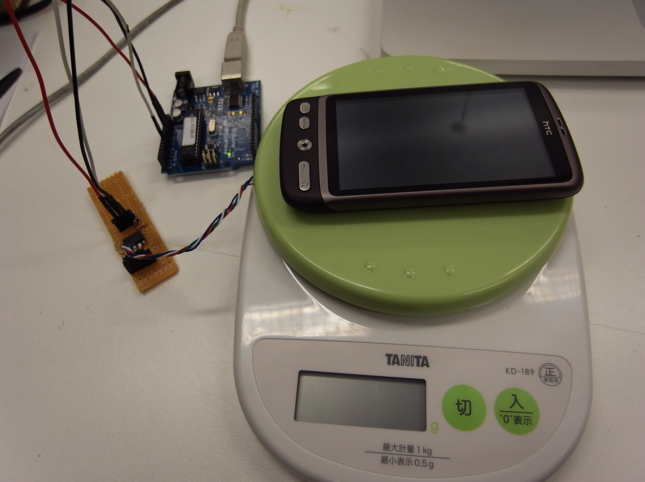
\includegraphics[height=50mm]{img/sensor.png}
  \end{center}
  \caption{重さを計るセンサーの試作版}
  \ecaption{prototype of sensor to detect weight}
  \label{fig:sensor}
\end{figure}

\begin{figure}
  \begin{center}
    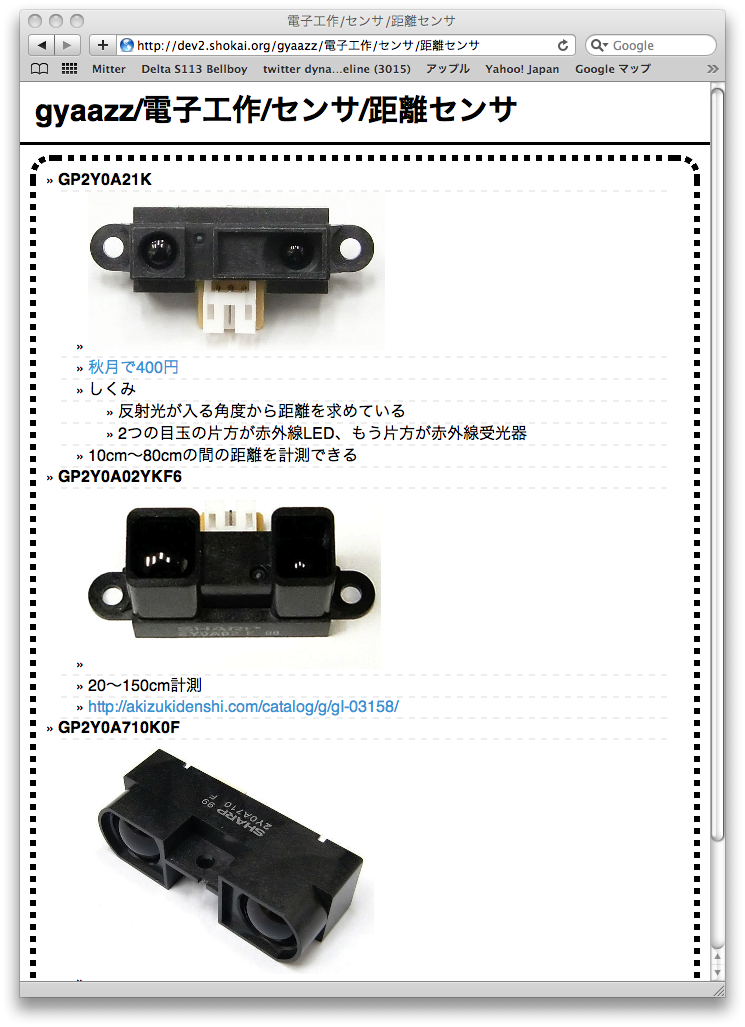
\includegraphics[height=100mm]{img/gyaazz.png}
  \end{center}
  \caption{ウェブアプリケーション gyaazz}
  \ecaption{gyaazz : outline editor web application}
  \label{fig:gyaazz}
\end{figure}

\begin{figure}
  \begin{center}
    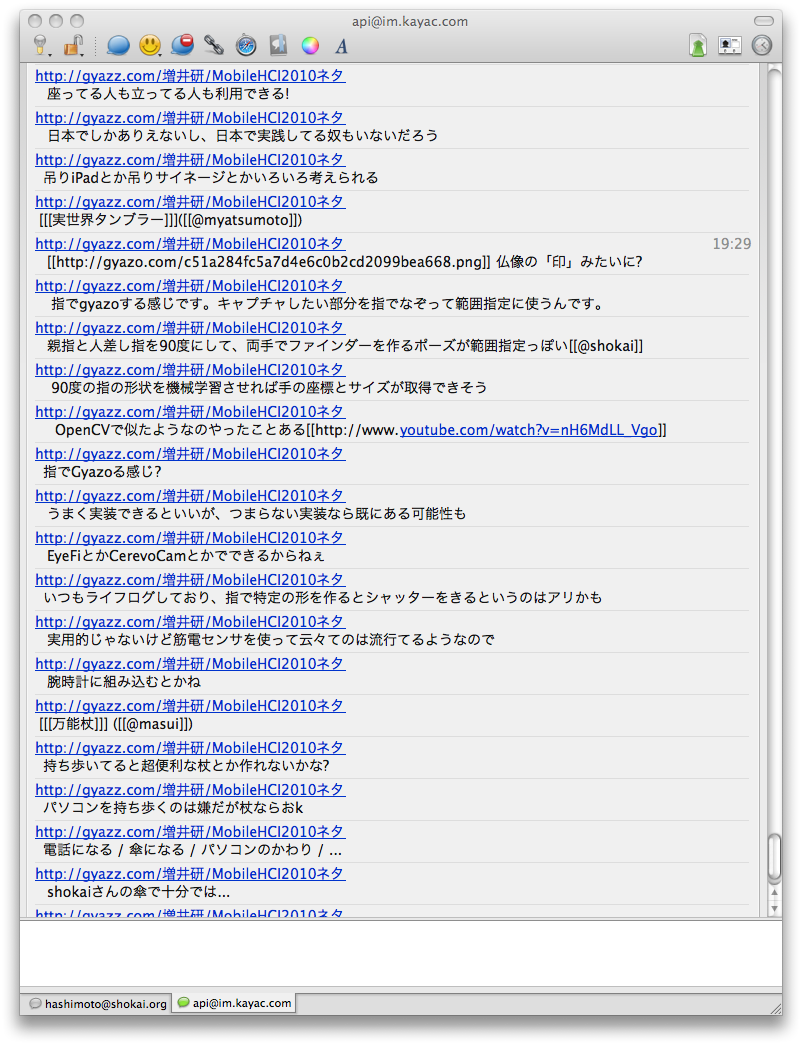
\includegraphics[height=80mm]{img/gyazz-checker.png}
  \end{center}
  \caption{google talk上でのgyazz-checker}
  \ecaption{gyaazz-checker on google talk}
  \label{fig:checker}
\end{figure}

\begin{figure}
  \begin{center}
    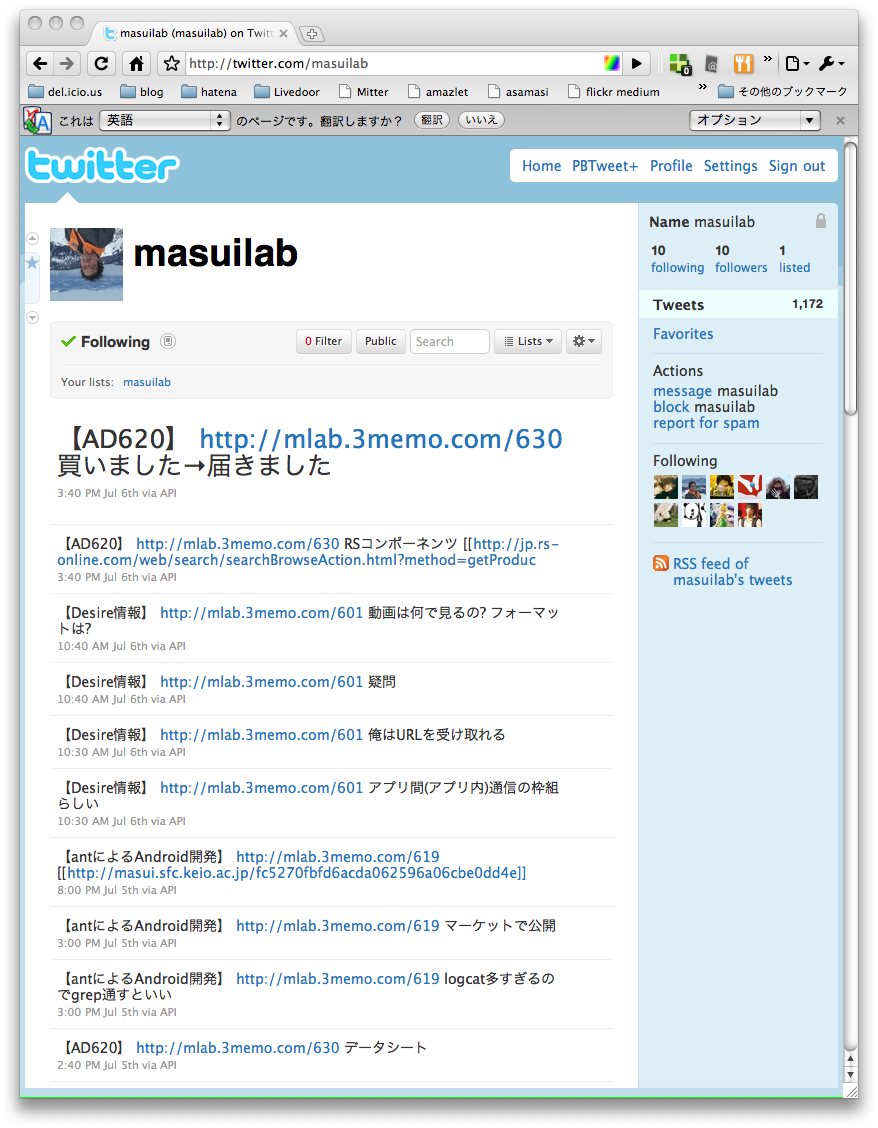
\includegraphics[height=90mm]{img/gyazz-twitter.png}
  \end{center}
  \caption{twitter上でのgyazz-checker}
  \ecaption{gyaazz-checker on twitter}
  \label{fig:twitter}
\end{figure}

\section{システムの実装}
はかりがある.Arduinoで重さ読む.重さとIDのDBを参照してwikiページを開く.DBはmongod.wikiはsinatraとtokyocabinetでできている.wikiの更新は定期的にtwitterとiPhoneとAndroidとIMに流れる.便利!!
githubへのリンクを貼りまくろう.はかりとか更新通知の精度・速度については適当に書く.


\section{まとめ}
重さで物体認識してweb上の情報と関連付け,wikiも作って,通知機能も作った.便利である.
